\subsection{Дерево}

\begin{defn}
    Лес --- граф без циклов.
\end{defn}

\begin{defn}
    Дерево --- связный граф без циклов.
\end{defn}

\begin{defn}
    Ориентированное дерево --- орграф без циклов, в котором только одна вершина имеет нулевую степень захода, а все остальные вершины имеют степень захода $1$.
\end{defn}

Вершина с нулевой степенью захода --- корень дерева, 

вершины с нулевой степенью исхода --- листья.

\begin{center}
    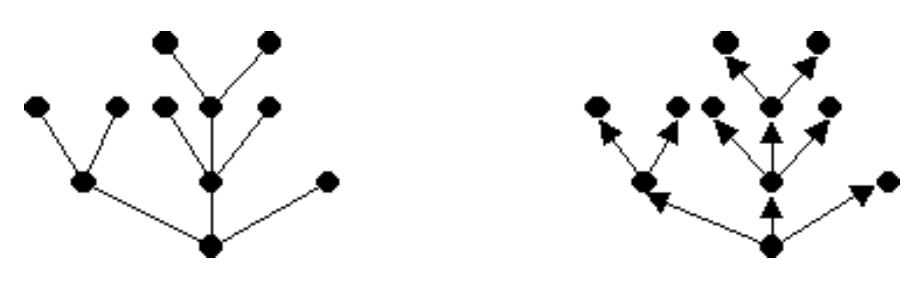
\includegraphics[width=0.5\textwidth]{par21tree.png}
\end{center}